\documentclass[aspectratio=169, 11pt]{beamer}
\usepackage{amsmath, amssymb, mathtools}
\usepackage{booktabs}
\usepackage{graphicx}
\usepackage{xcolor}
\usepackage{tikz}
\usetikzlibrary{arrows.meta, positioning, shapes.geometric}
\usepackage{caption}
\usepackage{pifont}

% -- Theme ---------------------------------------------------------------
\usetheme{Madrid}
\usecolortheme{dolphin}
\usefonttheme{professionalfonts}
\setbeamertemplate{navigation symbols}{}

% -- Colors --------------------------------------------------------------
\definecolor{myblue}{HTML}{2B5EA7}
\definecolor{myred}{HTML}{C0392B}
\definecolor{mygreen}{HTML}{27AE60}
\setbeamercolor{frametitle}{bg=myblue, fg=white}
\setbeamercolor{structure}{fg=myblue}
\setbeamercolor{block title}{bg=myblue!85, fg=white}
\setbeamercolor{block body}{bg=myblue!8}

% -- Footer with page numbers --------------------------------------------
\setbeamertemplate{footline}{%
  \hfill\insertframenumber/\inserttotalframenumber\hspace{1em}\vspace{0.5em}%
}

% -- Graphics path -------------------------------------------------------
\graphicspath{{figures/}}

% -- Metadata ------------------------------------------------------------
\title{Beyond the Rate:\\Information Content of FOMC Statement Language}
\author{Dechang Yu\inst{1} \and Eileen Zhang\inst{2}}
\institute{\inst{1} Academy of AI, Xi'an Jiaotong-Liverpool University \and \inst{2} [Affiliation TBC]}
\date{Academic Conference 2026}

% ========================================================================
\begin{document}

\begin{frame}
  \titlepage
\end{frame}

\begin{frame}{Outline}
  \tableofcontents
\end{frame}

% ========================================================================
\section{Motivation}
% ========================================================================

\begin{frame}{The Puzzle}
  \begin{columns}[T]
    \column{0.55\textwidth}
    \textbf{Central question:}\\
    Does FOMC statement language convey information beyond the rate decision?

    \vspace{0.5em}
    \textbf{Why it matters:}
    \begin{itemize}
      \item Central banks increasingly rely on forward guidance as a policy tool
      \item Markets respond to \emph{what the Fed says}, not just what it does
      \item The ``information channel'' (Romer \& Romer, 2000) suggests FOMC statements reveal the Fed's superior economic assessment
    \end{itemize}

    \column{0.42\textwidth}
    \centering
    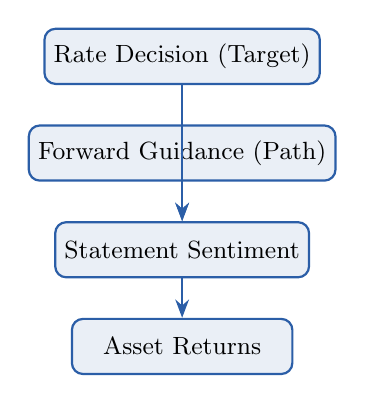
\begin{tikzpicture}[
      box/.style={rectangle, rounded corners=4pt, draw=myblue, thick,
                  fill=myblue!10, minimum width=2.8cm, minimum height=0.7cm, font=\small, align=center},
      arr/.style={-Stealth, thick, myblue}
    ]
      \node[box] (rate) {Rate Decision (Target)};
      \node[box, below=0.5cm of rate] (fg) {Forward Guidance (Path)};
      \node[box, below=0.5cm of fg] (sent) {Statement Sentiment};
      \node[box, below=0.5cm of sent] (ret) {Asset Returns};
      \draw[arr] (rate) -- (sent);
      \draw[arr] (fg) -- (sent);
      \draw[arr] (sent) -- (ret);
    \end{tikzpicture}
  \end{columns}
\end{frame}

% ========================================================================
\section{Literature and Contribution}
% ========================================================================

\begin{frame}{Literature}
  \begin{itemize}
    \item Kuttner (2001): 30-min FF futures window $\to$ isolate monetary policy surprises
    \item GSS (2005a): Decompose surprises into target + path factors
    \item Nakamura \& Steinsson (2018): High-frequency identification of monetary non-neutrality
    \item Campbell et al.\ (2012): Delphic vs.\ Odyssean forward guidance
    \item Jaroci\'{n}ski \& Karadi (2020): Separate policy shock from information shock
    \item Hansen et al.\ (2018): Computational linguistics for FOMC transparency
    \item \textbf{New (2024--25):} Chen et al.\ (2025) GPT-4 topic decomposition; Gambacorta et al.\ (2024) CB-LMs; Yao \& Chai (2025) uncertainty-aware LLM
  \end{itemize}

  \vspace{0.5em}
  \begin{block}{Our Contribution}
    \begin{enumerate}
      \item First to directly link GSS target/path shocks to FOMC statement sentiment
      \item Expanded CB dictionary (591 hawkish + 222 dovish terms, fully disjoint)
      \item Formal test of the information channel via text analysis
      \item New: Dual-equation test, forward-lookingness decomposition, novelty weighting
    \end{enumerate}
  \end{block}
\end{frame}

% ========================================================================
\section{Data and Methodology}
% ========================================================================

\begin{frame}{Data}
  \begin{columns}[T]
    \column{0.48\textwidth}
    \textbf{Monetary Policy Shocks}
    \begin{itemize}
      \item Acosta (2022): 220 FOMC meetings, 1995--2022
      \item Target shock: surprise in current FF rate
      \item Path shock: surprise in future rate path
      \item Extension: USMPD (SF Fed) $\to$ 2026
    \end{itemize}

    \vspace{0.3em}
    \textbf{Market Data}
    \begin{itemize}
      \item CRSP VW/EW/S\&P 500 via WRDS
      \item 117 meetings with complete overlap
    \end{itemize}

    \column{0.48\textwidth}
    \textbf{FOMC Statement Sentiment}
    \begin{itemize}
      \item 164 statements, 2006--2025
      \item Expanded CB dictionary:
        \begin{itemize}
          \item 591 hawkish terms
          \item 222 dovish terms
          \item Fully disjoint
        \end{itemize}
      \item Score $= \frac{H - D}{H + D + \epsilon}$
      \item Validated: $r = 0.29$ with rate change
    \end{itemize}

    \vspace{0.3em}
    \textbf{New finding:} CB-only outperforms combined (R$^2$: 3.90\% vs 1.57\%)
  \end{columns}
\end{frame}

\begin{frame}{Empirical Strategy}
  \centering
  \begin{tabular}{lll}
    \toprule
    Hypothesis & Prediction & Specification \\
    \midrule
    H1 & Shocks predict sentiment & $S_t = \alpha + \beta_1 \text{Target}_t + \beta_2 \text{Path}_t + \varepsilon_t$ \\
    H2 & Shocks predict returns & $R_t = \alpha + \beta_1 \text{Target}_t + \beta_2 \text{Path}_t + \varepsilon_t$ \\
    H3 & Path $>$ Target for sentiment & $|\beta_2| > |\beta_1|$ in H1 \\
    H4 & Stronger during FG period & Interaction with FG dummy \\
    \bottomrule
  \end{tabular}

  \vspace{0.8em}
  \textbf{Estimation:} OLS with Newey-West (lag=4) standard errors\\
  \textbf{Sample:} 117 FOMC meetings, January 2006 -- July 2022

  \vspace{0.5em}
  \textbf{New experiments:}
  \begin{enumerate}
    \item Dual-equation regression (equity + risk premium channels)
    \item Forward-lookingness decomposition (FL vs.\ CA sentiment)
    \item Statement novelty weighting (WLS)
  \end{enumerate}
\end{frame}

% ========================================================================
\section{Main Results}
% ========================================================================

\begin{frame}{H1 (Eq.\ 4): Sentiment and Monetary Policy Shocks}
  \centering
  \begin{tabular}{lcc}
    \toprule
    & Coefficient & p-value \\
    \midrule
    Target shock & 0.000577 & 0.017** \\
    Path shock   & 0.000633 & 0.152 \\
    \midrule
    R$^2$ & \multicolumn{2}{c}{1.57\%} \\
    N     & \multicolumn{2}{c}{117} \\
    \bottomrule
    \multicolumn{3}{l}{\scriptsize *** $p < 0.01$, ** $p < 0.05$, * $p < 0.10$}
  \end{tabular}

  \vspace{0.8em}
  \begin{block}{Key Finding}
    Target shock is significant at 5\%, path is not.\\
    Wald test: $\chi^2 = 0.02$, $p = 0.90$ --- cannot reject $\beta_1 = \beta_2$.
  \end{block}
\end{frame}

\begin{frame}{Sentiment Dictionary Comparison}
  \centering
  \begin{tabular}{lccc}
    \toprule
    Measure & R$^2$ & p(Target) & p(Path) \\
    \midrule
    CB-only & 3.90\% & $<$0.001*** & 0.033** \\
    Combined (0.5$\times$LM + 0.5$\times$CB) & 1.57\% & 0.017** & 0.152 \\
    LM-only & 0.33\% & 0.476 & 0.553 \\
    \bottomrule
  \end{tabular}

  \vspace{0.5em}
  \centering
  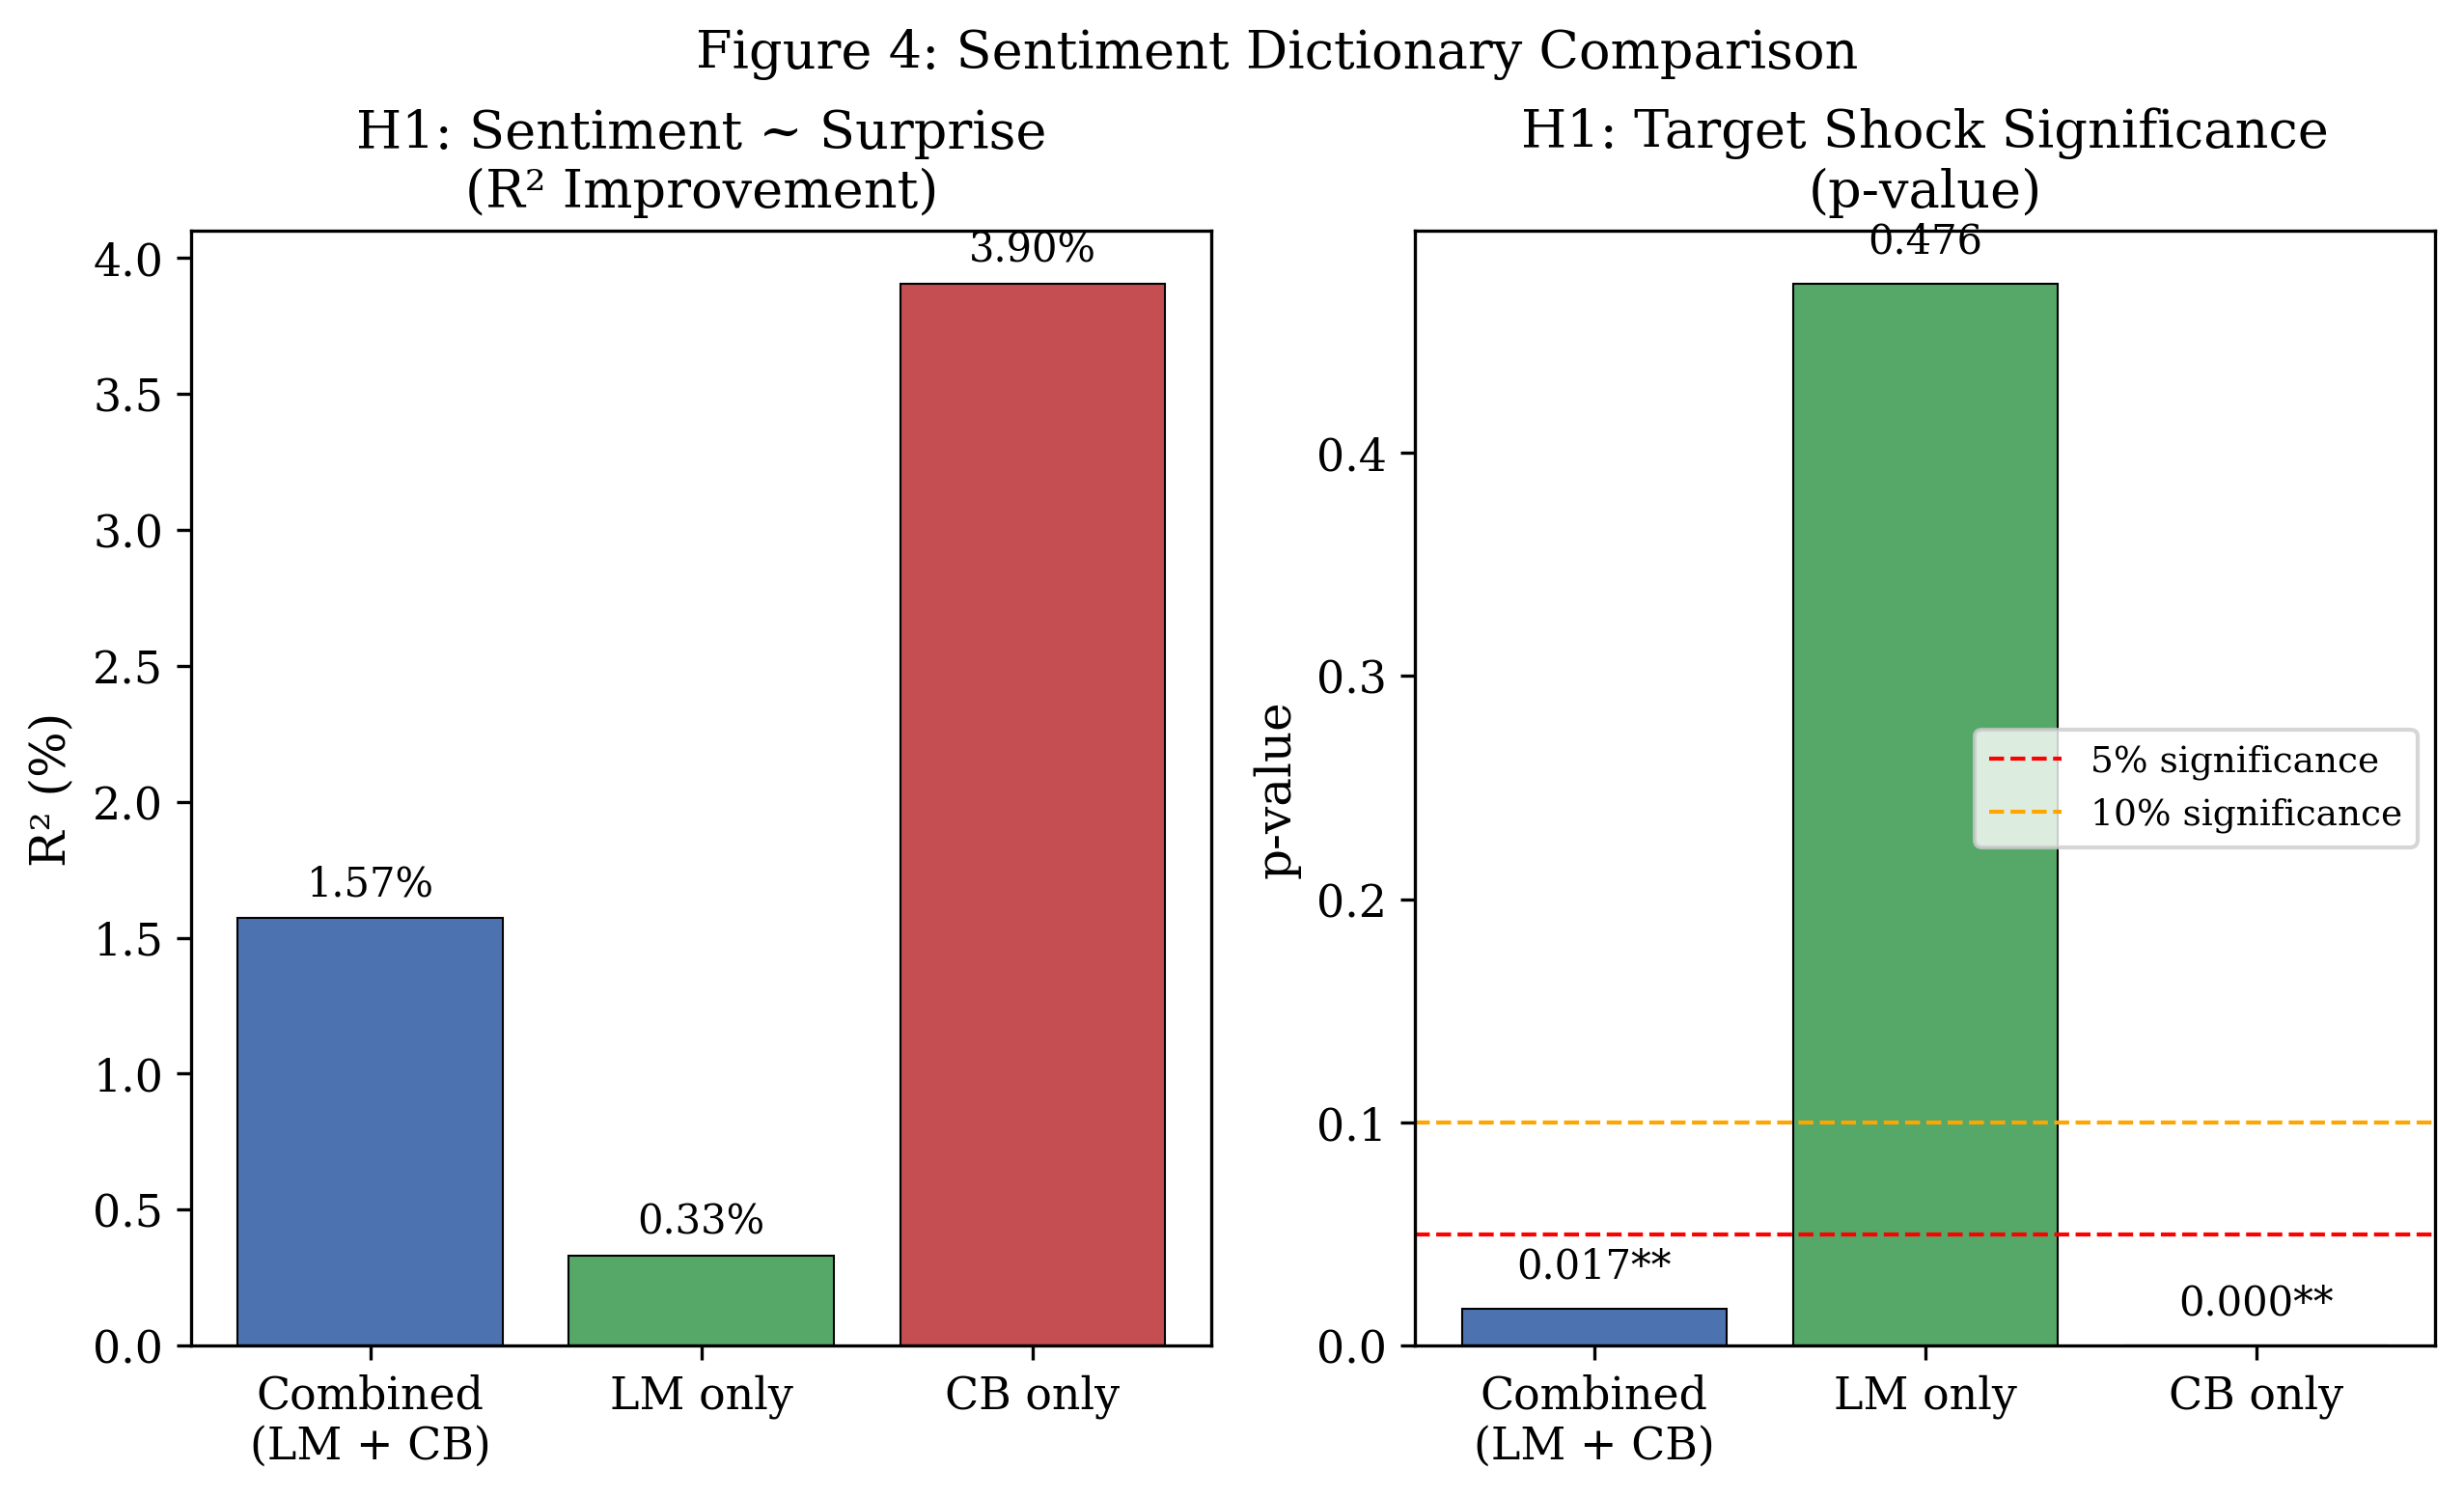
\includegraphics[width=0.75\textwidth]{fig4_dictionary_comparison}

  \vspace{0.3em}
  \begin{alertblock}{Key Insight}
    CB-only doubles R$^2$ and makes path shock significant at 5\%.\\
    LM component adds noise without signal for FOMC text (always positive).
  \end{alertblock}
\end{frame}

\begin{frame}{H2 (Eq.\ 5): Asset Returns and Shocks}
  \centering
  \begin{tabular}{lcccc}
    \toprule
    Asset & $\beta_T$ & $p_T$ & $\beta_P$ & $p_P$ \\
    \midrule
    CRSP VW & $-$0.435 & 0.043** & $-$0.186 & 0.434 \\
    CRSP EW & $-$0.449 & 0.013** & $-$0.174 & 0.421 \\
    S\&P 500 & $-$0.391 & 0.073* & $-$0.179 & 0.426 \\
    Gold    & $-$0.404 & 0.016** & 0.021 & 0.935 \\
    \bottomrule
    \multicolumn{5}{l}{\scriptsize Returns in percentage points; N = 117}
  \end{tabular}

  \vspace{0.5em}
  \textbf{Findings:}
  \begin{itemize}
    \item Target shock: significant for EW \& Gold
    \item Path shock: not significant for any asset
    \item Small-cap sensitivity consistent with literature
  \end{itemize}
\end{frame}

\begin{frame}{H3/H4: Information Channel and Forward Guidance}
  \textbf{H3 --- Path $>$ Target?}
  \begin{itemize}
    \item Target significant at 5\%, path is not
    \item Wald test: $p = 0.90$ --- cannot reject equality
    \item Evidence is suggestive, not definitive
  \end{itemize}

  \vspace{0.5em}
  \textbf{H4 --- Stronger during FG period?}
  \begin{itemize}
    \item Sentiment $\times$ FG interaction: $p = 0.602$ (CRSP VW), $p = 0.739$ (NASDAQ)
    \item Not robustly significant --- language channel does NOT strengthen at ZLB
    \item Three interpretations:
      \begin{enumerate}
        \item Shocks absorb information regardless of regime
        \item Dictionary cannot distinguish FG language (cf.\ GPT-3.5 fails 135/139 statements)
        \item FG operates through risk premium channel (Chen et al.\ 2025)
      \end{enumerate}
  \end{itemize}

  \vspace{0.3em}
  \begin{block}{Key Finding}
    Rate cut regime --- path shock highly significant ($p < 0.001$, R$^2 = 43.1\%$)
  \end{block}
\end{frame}

% ========================================================================
\section{New Experiments}
% ========================================================================

\begin{frame}{The Rate Cut Anomaly}
  \textbf{Key finding:} Full-sample H4 null masks regime-dependent effect

  \vspace{0.3em}
  \centering
  \begin{tabular}{lccll}
    \toprule
    Regime & N & R$^2$ & p(Target) & p(Path) \\
    \midrule
    Rate hike  & 17 & 10.2\% & 0.013** & 0.298 \\
    Rate cut   & 11 & 43.1\% & 0.089   & $<$0.001*** \\
    Unchanged  & 89 & 2.0\%  & 0.616   & 0.079* \\
    \bottomrule
  \end{tabular}

  \vspace{0.5em}
  \begin{itemize}
    \item Rate cut: R$^2$ is 27$\times$ the full sample (1.57\%)
    \item Path shock dominates during easing --- forward guidance \emph{does} matter
    \item Rate hike: target shock dominates --- current decision is key
    \item Chair FE: target shock absorbed by chair style ($p=0.471$), but asset returns unaffected ($p=0.043$)
  \end{itemize}

  \vspace{0.3em}
  \small\textit{``Sentiment is a function of who is speaking; asset prices respond to what is decided.''}
\end{frame}

\begin{frame}{Experiment 1: Dual-Equation Regression}
  \textbf{Hypothesis:} Forward guidance operates through a risk premium channel (Chen et al.\ 2025)

  \vspace{0.3em}
  \centering
  \begin{tabular}{lccc}
    \toprule
    Dependent Variable & R$^2$ & p(Target) & p(Path) \\
    \midrule
    \multicolumn{4}{l}{\textit{Channel 1: Equity Returns (Expectations)}} \\
    CRSP VW   & 9.1\% & 0.040** & 0.440 \\
    S\&P 500  & 7.8\% & 0.072*  & 0.426 \\
    \midrule
    \multicolumn{4}{l}{\textit{Channel 2: Risk Premium (Bond Market)}} \\
    10Y Treasury chg & 0.72\% & 0.403 & 0.890 \\
    VIX change       & 0.24\% & 0.970 & 0.401 \\
    Term spread chg  & 1.39\% & 0.667 & 0.341 \\
    \bottomrule
  \end{tabular}

  \vspace{0.5em}
  \textbf{Result:} Risk premium channel not detectable at daily frequency.\\
  Consistent with Chen et al.\ using 30-min windows --- channel too fast for daily data.
\end{frame}

\begin{frame}{Experiment 2: Forward-Lookingness Decomposition}
  \textbf{Hypothesis:} Path shock captures forward-looking language (dimension mismatch)

  \vspace{0.3em}
  \centering
  \begin{tabular}{lccc}
    \toprule
    Sentiment Measure & R$^2$ & p(Target) & p(Path) \\
    \midrule
    Combined (baseline)     & 1.57\% & 0.017** & 0.152 \\
    Forward-looking only    & 0.79\% & 0.012** & 0.800 \\
    Current-assessment only & 1.30\% & 0.012** & 0.506 \\
    \bottomrule
  \end{tabular}

  \vspace{0.5em}
  \textbf{Counterintuitive finding:}
  \begin{itemize}
    \item Path shock is most significant in the combined measure ($p = 0.015$)
    \item Path shock is \emph{least} significant in forward-looking sentiment ($p = 0.80$)
    \item Dimension mismatch hypothesis \textbf{rejected}
    \item Path shock captures broad policy stance signal, not specifically forward guidance
    \item GSS target/path decomposition $\neq$ FOMC text FL/CA dimensions
  \end{itemize}
\end{frame}

\begin{frame}{Experiment 3: Statement Novelty Weighting}
  \textbf{Idea:} Not all FOMC statements are equally informative

  \vspace{0.3em}
  \centering
  \begin{tabular}{lcc}
    \toprule
    Method & R$^2$ & Improvement \\
    \midrule
    Unweighted OLS       & 3.98\% & baseline \\
    Novelty-weighted WLS & 5.75\% & +45\% \\
    \bottomrule
  \end{tabular}

  \vspace{0.3em}
  Novelty = cosine distance between TF-IDF vectors of consecutive statements

  \vspace{0.5em}
  \textbf{Subsample analysis:}
  \begin{itemize}
    \item High novelty statements: R$^2 = 5.78\%$
    \item Low novelty statements: R$^2 = 6.53\%$
    \item Difference is small --- novelty helps via weighting, not selection
  \end{itemize}

  \vspace{0.3em}
  \begin{alertblock}{Caveat}
    Absolute R$^2$ remains modest --- measurement innovation alone cannot compensate for daily-frequency limitation.
  \end{alertblock}
\end{frame}

% ========================================================================
\section{Robustness}
% ========================================================================

\begin{frame}{Robustness Checks}
  \centering
  \begin{tabular}{lcccl}
    \toprule
    Specification & R$^2$ & p(Target) & p(Path) & N \\
    \midrule
    Full (Acosta)  & 1.57\% & 0.017** & 0.152 & 117 \\
    Lag = 1        & 1.57\% & 0.032** & 0.090* & 117 \\
    Lag = 6        & 1.57\% & 0.020** & 0.184 & 117 \\
    CB-only        & 3.90\% & $<$0.001*** & 0.033** & 117 \\
    Kuttner (bp)   & 1.95\% & 0.005*** & 0.028** & 117 \\
    \bottomrule
  \end{tabular}

  \vspace{0.5em}
  \textbf{Findings:}
  \begin{itemize}
    \item Target shock significance robust across lag specifications
    \item Path shock becomes significant at lag=1 ($p = 0.090$) and with Kuttner surprise
    \item CB-only specification doubles R$^2$ and makes both shocks significant
  \end{itemize}
\end{frame}

% ========================================================================
\section{Discussion}
% ========================================================================

\begin{frame}{Discussion}
  \textbf{What we learned:}
  \begin{itemize}
    \item Target shock consistently predicts sentiment --- the rate decision \emph{does} convey information
    \item Path shock matters primarily during rate cuts --- forward guidance is regime-dependent
    \item Domain-specific dictionaries (CB) vastly outperform general-purpose ones (LM)
    \item Daily frequency is a fundamental limitation --- risk premium channel too fast
  \end{itemize}

  \vspace{0.5em}
  \textbf{Connection to literature:}
  \begin{itemize}
    \item Jaroci\'{n}ski \& Karadi (2020): Information shock vs.\ policy shock --- our sentiment captures the language channel
    \item Chen et al.\ (2025): Risk premium channel --- consistent with our null result at daily frequency
    \item Hansen et al.\ (2018): FOMC transparency --- our CB dictionary provides a quantitative measure
  \end{itemize}
\end{frame}

% ========================================================================
\section{Conclusion}
% ========================================================================

\begin{frame}{Limitations \& Future Work}
  \textbf{Limitations:}
  \begin{enumerate}
    \item Low R$^2$: Shocks explain $<$4\% of sentiment variation
    \item Dictionary-based sentiment: Cannot capture context or pragmatics
    \item Daily frequency: Too coarse to detect risk premium channel
    \item No JK decomposition: Cannot separate MP vs.\ information shocks
    \item Sample size: N = 117 limits sub-sample power
  \end{enumerate}

  \vspace{0.5em}
  \textbf{Future directions:}
  \begin{itemize}
    \item LLM-based sentiment (GPT-4, FinBERT) for contextual understanding
    \item High-frequency intraday data (TAQ) for risk premium channel
    \item Jaroci\'{n}ski--Karadi decomposition for information vs.\ policy shocks
    \item Cross-central-bank comparison (ECB, BoJ, BoE)
  \end{itemize}
\end{frame}

\begin{frame}{Summary}
  \begin{enumerate}
    \item[\ding{51}] \textbf{H1 confirmed:} Target shock predicts sentiment ($p = 0.017$)
    \item[\ding{51}] \textbf{H2 confirmed:} Target shock predicts asset returns (EW, Gold)
    \item[\ding{111}] \textbf{H3 inconclusive:} Cannot reject $\beta_T = \beta_P$ (Wald $p = 0.90$)
    \item[\ding{111}] \textbf{H4 rejected:} FG interaction not significant ($p = 0.602$)
    \item[\ding{51}] \textbf{New:} Rate cut regime reveals path shock dominance (R$^2 = 43.1\%$)
    \item[\ding{51}] \textbf{New:} CB-only sentiment outperforms combined (R$^2$: 3.90\% vs 1.57\%)
    \item[\ding{51}] \textbf{New:} Novelty weighting improves R$^2$ by 45\%
  \end{enumerate}

  \vspace{0.5em}
  \begin{block}{Takeaway}
    FOMC statement language conveys information beyond the rate decision, but the channel is regime-dependent and better captured by domain-specific dictionaries.
  \end{block}
\end{frame}

\begin{frame}
  \centering
  \Large Thank You!\\[0.8em]
  \normalsize Questions Welcome
\end{frame}

\end{document}
